%Copyright 2014 Jean-Philippe Eisenbarth
%This program is free software: you can
%redistribute it and/or modify it under the terms of the GNU General Public
%License as published by the Free Software Foundation, either version 3 of the
%License, or (at your option) any later version.
%This program is distributed in the hope that it will be useful,but WITHOUT ANY
%WARRANTY; without even the implied warranty of MERCHANTABILITY or FITNESS FOR A
%PARTICULAR PURPOSE. See the GNU General Public License for more details.
%You should have received a copy of the GNU General Public License along with
%this program.  If not, see <http://www.gnu.org/licenses/>.

%Based on the code of Yiannis Lazarides
%http://tex.stackexchange.com/questions/42602/software-requirements-specification-with-latex
%http://tex.stackexchange.com/users/963/yiannis-lazarides
%Also based on the template of Karl E. Wiegers
%http://www.se.rit.edu/~emad/teaching/slides/srs_template_sep14.pdf
%http://karlwiegers.com
\documentclass{scrreprt}
\usepackage{listings}
\usepackage{underscore}
\usepackage[bookmarks=true]{hyperref}
\usepackage[utf8]{inputenc}
\usepackage[english]{babel}
\usepackage{graphicx}
\hypersetup{
    bookmarks=false,    % show bookmarks bar?
    pdftitle={Software Requirement Specification},    % title
    pdfauthor={Jean-Philippe Eisenbarth},                     % author
    pdfsubject={TeX and LaTeX},                        % subject of the document
    pdfkeywords={TeX, LaTeX, graphics, images}, % list of keywords
    colorlinks=true,       % false: boxed links; true: colored links
    linkcolor=blue,       % color of internal links
    citecolor=black,       % color of links to bibliography
    filecolor=black,        % color of file links
    urlcolor=purple,        % color of external links
    linktoc=page            % only page is linked
}%
\def\myversion{1.0 }
\date{}
%\title
\usepackage{hyperref}
\begin{document}

\begin{flushright}
    \rule{16cm}{5pt}\vskip1cm
    \begin{bfseries}
        \Huge{SOFTWARE REQUIREMENTS\\ SPECIFICATION}\\
        \vspace{1.5cm}
        for\\
        \vspace{1.5cm}
        Condo Management System\\
        \vspace{1.5cm}
        \LARGE{Version \myversion}\\
        \vspace{1.5cm}
        Prepared by Mhaisdhune, Trupti Vishnu\\
        Peixoto Costa Neto, Mario\\
        Yohannan, Blessy\\
        Zhang, Xuezhu\\
        \vspace{1.5cm}
        Texas State University\\
        \vspace{1.5cm}
        \today\\
    \end{bfseries}
\end{flushright}

\tableofcontents

\chapter{Introduction}

\section{Purpose}
The purpose of this document is to present a detailed description of the Condo Management System, a system designed to manage clients, condos, tenants, units and debts and provide organized records of each tenant debts and emit notices for those debts. It will explain the functions that the manager will be able to access, the interfaces of the system, what the system will do, the constraints under which it must operate and how it will react to external stimuli. This document is intended for both users and developers of the system and will be submitted to the customer for approval.

\section{Problem statement}
A law office works as a representative of several condominium administration companies. These companies may have several hundreds tenants who rents their apartments and it’s very common for those tenants to skip rental and administration payments of the condo. The administration company has its own information system, but the law office only receives a monthly report with the up-to-date debts for all condos and units.

The job of the law office is to look at the reports and find the tenants who are in debt for more than a certain time and notify them that they should contact the law office to settle their debts or expect to be sued. But having several companies as clients - each of them having several hundreds of tenants - can lead to a tremendous amount of labor, it’s just not doable.

Each client will provide a monthly debt report with condo names, units in debt, tenants in debt, and debts information and the law office will use that report to import the data into the database.

Then, the system shall provide a screen to help the law office to easily find who’s in debt, for how long they are in debt and how much they owe. That same interface shall allow the law office to choose the tenants to be notified. After choosing, the system shall generate all the notices and the envelope labels for mailing as PDFs.

After notifying the tenants, they may contact to negotiate a settlement or to pay the full amount. Then, the system shall provide a feature to mark those debts as paid.

\chapter{Overall Description}

\section{Product Perspective}
The Condo Management System is a new web-based application and does not depend or is a part of any other system. It has one actor: the manager. The manager needs a compatible web browser and internet access to access the system.

\section{Software Interfaces}
PostgreSQL will be used as a Database Management System for the Condo Management System.

Compatible web-browsers: Chrome, Firefox and Safari.

\section{Product Functions}

\subsection{Create Client}
\subsubsection{Description}

The manager creates a client (Condo Administration Company), entering information such as name, contact name, contact phone, address, default fine percentage and default interest percentage for late payment.

\subsubsection{Rationale}

This function will make the client available to the system in order to create the condominia managed by this client. That will be necessary to import the debts and keep an organized record.

\subsubsection{UI wireframe}
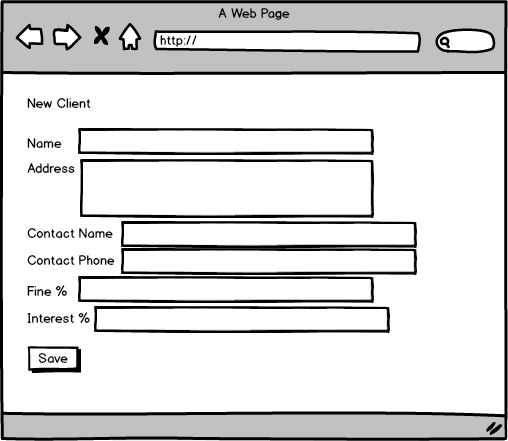
\includegraphics[scale=0.60]{mockups/createclient.png}

\subsection{Edit Client}
\subsubsection{Description}

The manager edits a client (Condo Administration Company), entering information such as name, contact name, contact phone, address, and default fine percentage and default interest percentage for late payment.

\subsubsection{Rationale}

This function will make possible to edit the client information whenever the data's changed or it was entered incorrectly. That's necessary to keep an organized record.

\subsubsection{UI wireframe}
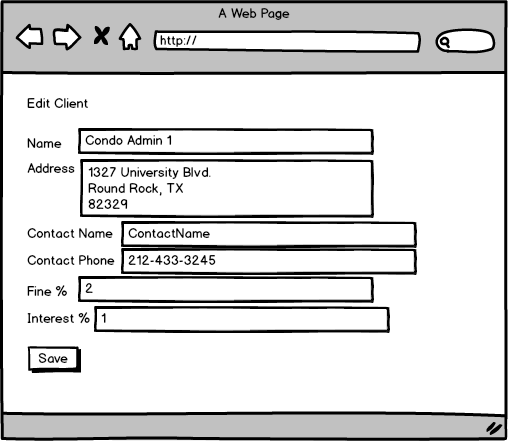
\includegraphics[scale=0.60]{mockups/editclient.png}

\subsection{Remove Client}
\subsubsection{Description}

The manager removes a client (Condo Administration Company) from the system.

\subsubsection{Rationale}

This function will make possible to remove the client from the system if the client decide to cancel the contract with the law firm. That's necessary to keep an organized record.

\subsection{Create Condo}
\subsubsection{Description}

The manager creates a condo, entering information such as name, address and chose the correct condo administration that manages it.

\subsubsection{Rationale}

This function will make the condo available to the system in order to create the units that belong to that condo. That will be necessary to import the debts and keep an organized record.

\subsubsection{UI wireframe}
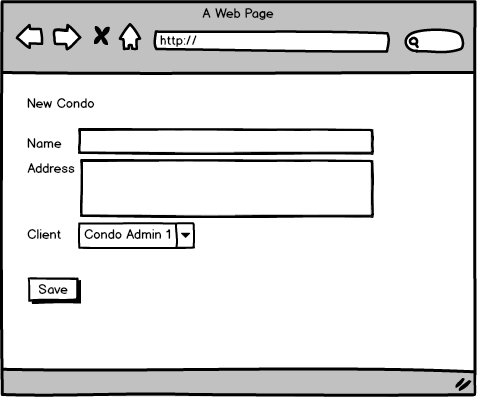
\includegraphics[scale=0.60]{mockups/createcondo.png}

\subsection{Edit Condo}
\subsubsection{Description}

The manager edits a condo, entering information such as name, address and chose the correct condo administration that manages it.

\subsubsection{Rationale}

This function will make possible to edit the condo information whenever the data's changed or it was entered incorrectly. That's necessary to keep an organized record.

\subsubsection{UI wireframe}
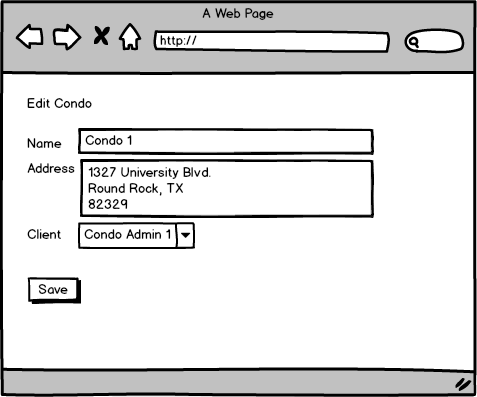
\includegraphics[scale=0.60]{mockups/editcondo.png}

\subsection{Remove Condo}
\subsubsection{Description}

The manager removes a condo from the system.

\subsubsection{Rationale}

This function will make possible to remove the condo from the system whenever the client decides it won't manage the debts from that condo anymore. That's necessary to keep an organized record.

\subsection{Create Unit}
\subsubsection{Description}

The manager creates an unit, entering information such as number, building name, select the correct condo that it belongs to, and the current tenant .

\subsubsection{Rationale}

This function will make the unit available to the system in order to assign the tenants and debts for that unit. That will be necessary to keep an organized record.

\subsubsection{UI wireframe}
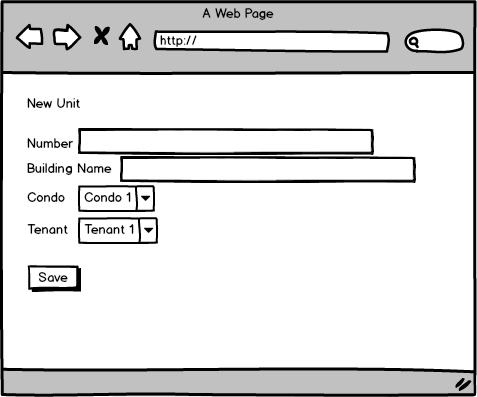
\includegraphics[scale=0.60]{mockups/createunit.png}

\subsection{Edit Unit}
\subsubsection{Description}

The manager edits an unit, entering information such as number, building name, the correct condo that it belongs to, and the current tenant.

\subsubsection{Rationale}

This function will make possible to edit the unit information whenever the data's changed or it was entered incorrectly. That's necessary to keep an organized record.

\subsubsection{UI wireframe}
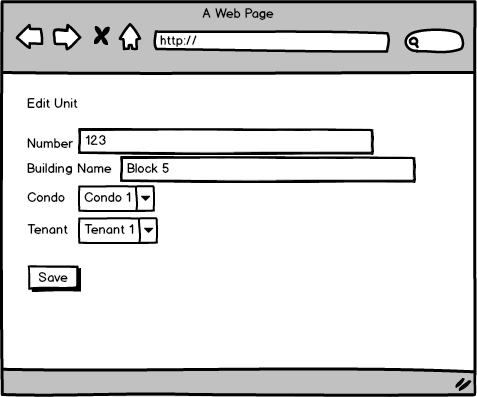
\includegraphics[scale=0.60]{mockups/editunit.png}

\subsection{Remove Unit}
\subsubsection{Description}

The manager removes an unit from the system.

\subsubsection{Rationale}

This function will make possible to remove the unit from the system whenever the client decides it won't manage the debts from that unit anymore. That's necessary to keep an organized record.

\subsection{Create Tenant}
\subsubsection{Description}

The manager creates a tenant, entering information such as name, billing address, SSN, phone number.

\subsubsection{Rationale}

This function will make the tenant available to the system in order to manage his debts. That will be necessary to keep an organized record.

\subsubsection{UI wireframe}
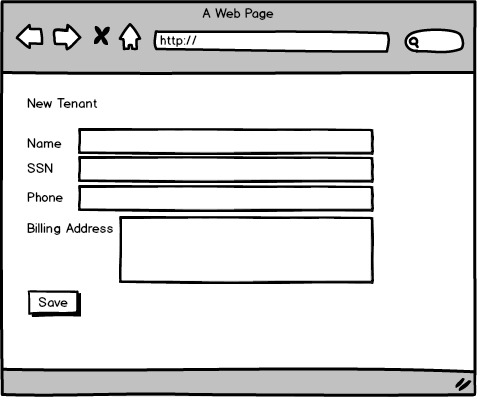
\includegraphics[scale=0.60]{mockups/createtenant.png}

\subsection{Edit Tenant}
\subsubsection{Description}

The manager edits a tenant, entering information such as name, billing address, SSN, phone number.

\subsubsection{Rationale}

This function will make possible to edit the tenant information whenever the data's changed or it was entered incorrectly. That's necessary to keep an organized record.

\subsubsection{UI wireframe}
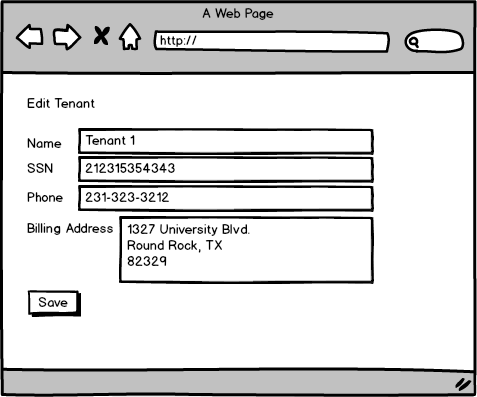
\includegraphics[scale=0.60]{mockups/edittenant.png}

\subsection{Remove Tenant}
\subsubsection{Description}

The manager removes a tenant from the system.

\subsubsection{Rationale}

This function will make possible to remove the tenant from the system whenever he's not needed anymore. That's necessary to keep an organized record.

\subsection{Create Debt}
\subsubsection{Description}

The manager creates a debt, entering information such as the unit in debt, description, original amount, due date, debt type (condo fee or extra fee).

\subsubsection{Rationale}

This function will make the debt available to the system in order to emit notices for it. That will be necessary to keep an organized record.

\subsubsection{UI wireframe}
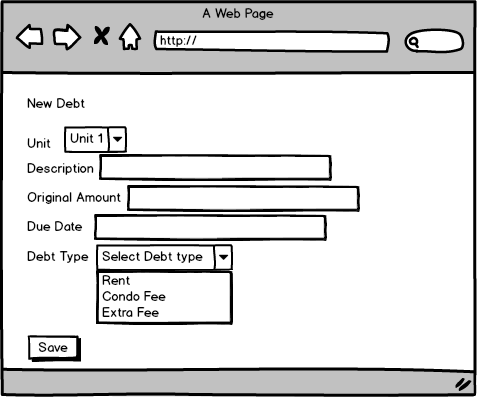
\includegraphics[scale=0.60]{mockups/createdebt.png}

\subsection{Edit Debt}
\subsubsection{Description}

The manager edit a debt, entering information such as the unit in debt, description, original amount, due date, debt type (condo fee or extra fee).

\subsubsection{Rationale}

This function will make possible to edit the debt information whenever the data's changed or it was entered incorrectly. That's necessary to keep an organized record.

\subsubsection{UI wireframe}
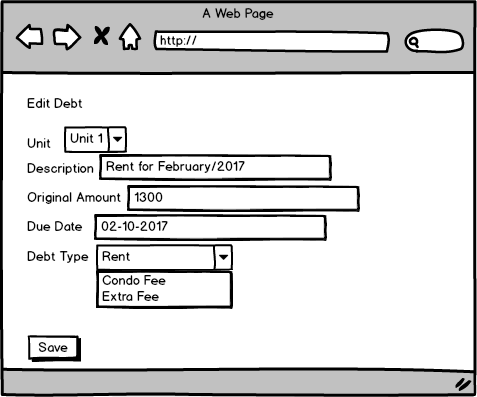
\includegraphics[scale=0.60]{mockups/editdebt.png}

\subsection{Remove Debt}
\subsubsection{Description}

The manager removes a debt from the system.

\subsubsection{Rationale}

This function will make possible to remove the debt from the system whenever it's not needed anymore or was incorrectly inserted in the system. That's necessary to keep an organized record.

\subsection{Create Notice}
\subsubsection{Description}

The manager creates a notice, entering information such as the tenant that needs to be notified and for which debts they are being notified.

\subsubsection{Rationale}

This function will make the notice available to the system in order to create the notice to be printed together with the envelope labels. That will be necessary to keep an organized record.

\subsubsection{UI wireframe}
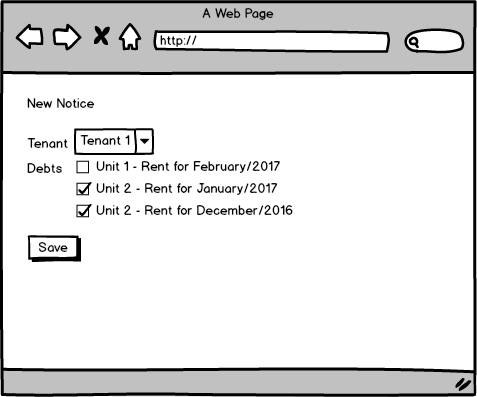
\includegraphics[scale=0.60]{mockups/createnotice.png}

\subsection{Edit Notice}
\subsubsection{Description}

The manager edits a notice, entering information such as the tenant that needs to be notified and for which debts they are being notified.

\subsubsection{Rationale}

This function will make possible to edit the notice information whenever the data's changed or it was entered incorrectly. That's necessary to keep an organized record.

\subsubsection{UI wireframe}
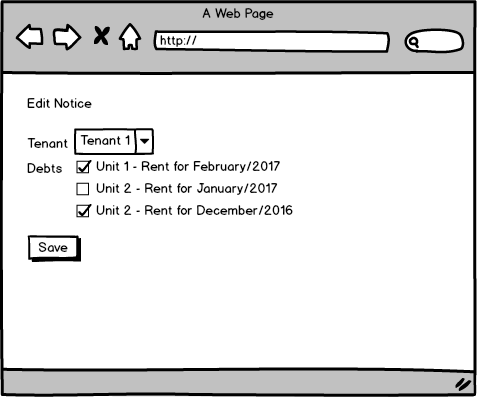
\includegraphics[scale=0.60]{mockups/editnotice.png}

\subsection{Remove Notice}
\subsubsection{Description}

The manager removes a notice from the system.

\subsubsection{Rationale}

This function will make possible to remove the notice from the system whenever it's not needed anymore or was incorrectly inserted in the system. That's necessary to keep an organized record.

\subsection{Import Monthly Report}
\subsubsection{Description}

The manager imports the monthly debt report provided by each client. The report contains the expanded outstanding debt for each unit for all condos managed by the client (Condo Administration Company).

\subsubsection{Rationale}

This function will make possible to import the monthly report data into the system in order to reconcile the system data with the outstanding debts and provide the option to emit notices for those debts.

\subsubsection{UI wireframe}
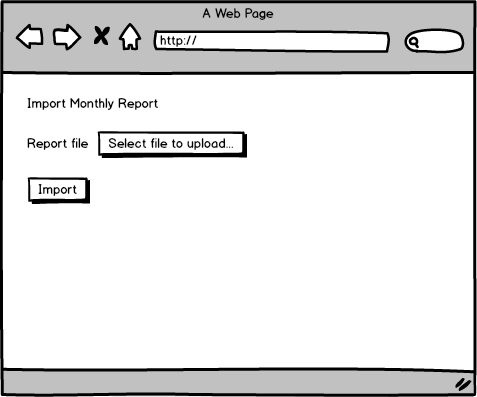
\includegraphics[scale=0.60]{mockups/importreport.png}

\chapter{Other Nonfunctional Requirements}

\section{Performance Requirements}
The system response time shall not exceed 10 seconds for any user interaction event.

\section{Reliability Requirements}
The application’s mean time between failures shall be at least 1 month.

\section{Robustness Requirements}
The application shall provide a meaningful error message and continue to operate properly when a human user provides incorrect inputs.

\section{Maintainability Requirements}
The average person-time required to make a minor enhancement (including testing and documentation update) shall not exceed one person week.

\section{Usability Requirements}
The application’s user interface shall be clear to its users.
Specifically, at least 70\% of a statistically valid sample of users shall rate the overall user interface as being either very clear or clear on the following scale (very clear, clear, neutral, unclear, very unclear).

\chapter{Constraints}

\section{Design}
The performance of the system depends on the underlying server and the database system.
Web page scaling depends on the device and the browser used.

\section{Implementation}
The system functionality depends on the ability to reliably transfer data over an active Internet connection. If the connection has high latency or bandwidth issues then the response time may be slower than desired.

\nocite{ieee}

\bibliographystyle{ieeetr}
\bibliography{srsbib}

\end{document}
